\documentclass[
  bibliography=totoc,     % Bibliography as unnumbered chapter in toc
  numbers=noenddot,       % No dot after figure/table number
  captions=tableheading,  % Correct spacing for table headings
  % titlepage=firstiscover, % Symmetrical margins on titlepage
  parskip=half,           % Hals skip instead of intend in new paragraph
  headings=normal,
  a4paper,
]{scrartcl}

% Warning, if another latex run is needed
\usepackage[aux]{rerunfilecheck}
\setcounter{tocdepth}{2}

%------------------------------------------------------------------------------
%-- Language and Type
%------------------------------------------------------------------------------
\usepackage{fontspec}
\defaultfontfeatures{Ligatures=TeX}  % -- becomes en-dash etc.

% Language: english | german
\usepackage{polyglossia}
\setdefaultlanguage{english}

% For german | english abstract and german | english titles in the toc
\setotherlanguages{english}

% Intelligent quotation marks, language and nesting sensitive
\usepackage[autostyle]{csquotes}

% Microtypographical features, makes the text look nicer on the small scale
\usepackage{microtype}

%------------------------------------------------------------------------------
%-- Math
%------------------------------------------------------------------------------
\usepackage{amsmath}
\usepackage{amssymb}
\usepackage{mathtools}

% Enable Unicode-Math and follow the ISO-Standards for typesetting math
\usepackage[
  math-style=ISO,
  bold-style=ISO,
  sans-style=italic,
  nabla=upright,
  partial=upright,
]{unicode-math}
\setmathfont{Latin Modern Math}

\usepackage{xfrac}   % Small fracs for the text with \sfrac{}{}
\usepackage{braket}  % Good for expectation values

%------------------------------------------------------------------------------
%-- Numbers and Units
%------------------------------------------------------------------------------
\usepackage[
  locale=US,
  separate-uncertainty=true,
  per-mode=symbol-or-fraction,
  exponent-product=\cdot,
]{siunitx}
\sisetup{math-micro=\text{µ},text-micro=µ}

%------------------------------------------------------------------------------
%--Tables
%------------------------------------------------------------------------------
\usepackage{booktabs}  % Use \toprule, \midrule, \bottomrule

%------------------------------------------------------------------------------
%-- Graphics
%------------------------------------------------------------------------------
\usepackage{graphicx}
\usepackage{grffile}

%------------------------------------------------------------------------------
%-- Colors
%------------------------------------------------------------------------------
\usepackage{xcolor}
\xdefinecolor{darkgrey}{HTML}{353132}
% Nord colors: https://github.com/arcticicestudio/nord
% Polar Night (dark greys)
\xdefinecolor{nordgrey1}{HTML}{2E3440}
\xdefinecolor{nordgrey2}{HTML}{3B4252}
\xdefinecolor{nordgrey3}{HTML}{434C5E}
\xdefinecolor{nordgrey4}{HTML}{4C566A}
% Snow Storm (muted whites)
\xdefinecolor{nordwhite1}{HTML}{D8DEE9}
\xdefinecolor{nordwhite2}{HTML}{E5E9F0}
\xdefinecolor{nordwhite3}{HTML}{ECEFF4}
% Frost (cool blues/greens)
\xdefinecolor{nordbluegreen}{HTML}{8FBCBB}
\xdefinecolor{nordcyan}{HTML}{88C0D0}
\xdefinecolor{nordpaleblue}{HTML}{81A1C1}
\xdefinecolor{norddeepblue}{HTML}{5E81AC}
% Aurora (muted accent colors)
\xdefinecolor{nordred}{HTML}{BF616A}
\xdefinecolor{nordorange}{HTML}{D08770}
\xdefinecolor{nordyellow}{HTML}{EBCB8B}
\xdefinecolor{nordgreen}{HTML}{A3BE8C}
\xdefinecolor{nordviolet}{HTML}{B48EAD}

%------------------------------------------------------------------------------
%-- Floats
%------------------------------------------------------------------------------
% Allow figures to be placed in the running text by default:
\usepackage{scrhack}
\usepackage{float}
\floatplacement{figure}{htbp}
\floatplacement{table}{htbp}

\usepackage[section, below]{placeins}  % Keep figures and tables in the section

\usepackage{caption}
\usepackage{subcaption}

%------------------------------------------------------------------------------
%-- Customize list environments
%------------------------------------------------------------------------------
\usepackage{enumitem}

%------------------------------------------------------------------------------
%-- Bibliography
%------------------------------------------------------------------------------
\usepackage[
  backend=biber,    % use modern biber backend
  autolang=hyphen,  % load hyphenation rules for if language of bibentry is not
                    % german, has to be loaded with \setotherlanguages
                    % in the references.bib use langid={en} for english sources
]{biblatex}

%------------------------------------------------------------------------------
%-- Code environment and verbatim
%------------------------------------------------------------------------------
\usepackage{listings}
\lstset{basicstyle=\ttfamily}
\newcommand{\code}[1]{\lstinline|#1|}

%------------------------------------------------------------------------------
%-- Misc
%------------------------------------------------------------------------------
\usepackage[pdfusetitle,unicode,]{hyperref}
\hypersetup{
  unicode=true,
  colorlinks,
  linkcolor=black,
  citecolor=black,
  filecolor=black,
  urlcolor=norddeepblue,
}
\usepackage{bookmark}
\usepackage[shortcuts]{extdash}
\usepackage{scrlayer-scrpage}  % For custom KOMA layout modifications

%------------------------------------------------------------------------------
%-- Custom math operators
%------------------------------------------------------------------------------

\newcommand{\mperiod}{\quad\text{.}}
\newcommand{\mcomma}{\quad\text{,}}
\newcommand{\mintertext}[1]{\quad\text{#1}\quad}

\renewcommand{\d}[1]{\mathrm{d}#1}
\newcommand{\del}[1]{\partial #1}
\newcommand{\dd}[2]{\frac{\d{#1}}{\d{#2}}}
\newcommand{\deldel}[2]{\frac{\partial #1}{\partial #2}}

\DeclareMathOperator{\rect}{rect}
\DeclareMathOperator{\diag}{diag}
\DeclareMathOperator{\trace}{trace}


% \addbibresource{references.bib}


\begin{document}

\begin{titlepage}
  \centering
  {\scshape\Large Analysis Note\par}
  \vspace{1.5cm}
  {\huge\bfseries Time Dependent Point Source Stacking Search Associated with HESE Track Events\par}
  \vspace{2cm}
  {\Large Thorben Menne\par}

  \vfill

  % Bottom of the page
  \textsc{Transients Working Group}\par
  \url{https://wiki.icecube.wisc.edu/index.php/Transients_Working_Group}\par
  \vspace{0.5cm}
  \textsc{Reviewers}\par
  \begin{tabular}{rl}
    \centering
    Collaboration: & Sandro Kopper (\href{mailto:sjkopper@ua.edu}{sjkopper@ua.edu}) \\
    Working Group: & Kevin Meagher (\href{mailto:kmeagher@ulb.ac.be}{kmeagher@ulb.ac.be}) \\
  \end{tabular}\par
  \vspace{0.5cm}
  \textsc{Contact}\par
  \begin{tabular}{rl}
    \centering
    Mail: & \href{mailto:thorben.menne@tu-dortmund.de}{thorben.menne@tu-dortmund.de} \\
    Slack: & @mennthor
  \end{tabular}\par
  \vspace{2cm}
  {\Large Last edit: \today\par}
\end{titlepage}



\section{Overview}
This analysis is searching for a stacked lower energy neutrino contribution at the HESE track event positions, which are treated as transient sources.
We test for 21 generic box time windows increasing in logarithmic time from 2 seconds to 5 days symmetrically around all sources.

For the physics motivation: IceCube couldn't find a significant point source so far despite many different analysis and efforts.
Prominent examples relevant for this is search are the \href{time integrated 7 year point source search} and the \href{HESE 6 year point source search}, both with no significant results.
But the HESE events on their own show a clear astrophysical signal and therefore should originate from some sources.
This analysis test if there is any clustering of lower energy neutrino events around the HESE locations, aiming to constrain various HESE emission models.
\textcolor{nordred}{Note: The model selection is currently reviewed}.

The analysis method is a time dependent unbinned likelihood approach similar to the so called \enquote{GRB Likelihood}.
Key features used here are:
\begin{itemize}
  \item Background is modelled using scrambled data
  \item Using time dependent spatial background PDFs
  \item Energy PDF is estimated from data and MC with fixed index $E^{-2}$ power law
\end{itemize}

For source and test data we use:
\begin{itemize}
  \item Source dataset: 6 years HESE track events, IC79 - IC86, 2015.
  \item Test dataset: 5 years PS tracks (IC79 - IC86, 2014) + 1 year GFU (IC86, 2015)
\end{itemize}

The wiki can be found at \url{https://wiki.icecube.wisc.edu/index.php/Transient_HESE_Stacking} and contains this analysis note.



\section{Software}
The analysis scripts are in a git repository and can be found at \path{/home/tmenne/analysis/hese_transient_stacking/analysis}.
Code is enumerated in the order of script execution, if someone wants to redo all analysis steps.
The branch for this analysis is \code{original_hese} which tests the 22 original HESE track events.

The main analysis software used is made from scratch in python with a small C++ back-end for time consuming work with inspiration from \href{http://code.icecube.wisc.edu/projects/icecube/browser/IceCube/sandbox/skylab}{skylab} and \href{http://code.icecube.wisc.edu/projects/icecube/browser/IceCube/sandbox/richman/grbllh}{grbllh}.
The software repository can be found at \path{/home/tmenne/software/tdepps}.
The branch used for the analysis is \code{new_structure}.



\section{Datasets}
This analysis used HESE track events as sources and point source and GFU samples as a test dataset.

\subsection{Sources}
For source positions, the 22 HESE track events from 6 years of HESE data are tested.
The list of events can be seen at the list of \href{https://wiki.icecube.wisc.edu/index.php/Analysis_of_pre-public_alert_HESE/EHE_events#HESE
}{pre-public alert HESE events}.
For each of these events detailed \href{http://software.icecube.wisc.edu/documentation/projects/millipede/index.html}{millipede} scans exist.
The best fit positions are taken from these maps for the tested source positions by converting the best fit pixel in local coordinates to equatorial coordinates using the \href{http://software.icecube.wisc.edu/documentation/projects/astro/index.html}{astro} module.

Unlike other point source searches the positions of the sources are not exactly known due to our reconstruction uncertainties.
To estimate the worsened sensitivity for that, the millipede scan maps are later used to inject source positions.
To make this computationally feasible, all maps are converted to equatorial coordinates with the convention $\mathrm{RA} = \phi$ and $\mathrm{DEC} = \pi - \theta$, where $\phi, \theta$ are \href{https://healpy.readthedocs.io/en/latest/}{healpy}'s internal coordinates.
Because of the way healpixels are defined this is not a bijective operation, because the number of pixels in a zenith / declination / $\theta$ band gets smaller to the poles.
So the maps are built by defining a new map with exact pixels in equatorial coordinates, which then get mapped to an interpolated local map.
This can introduce angular errors in the size of a pixel diameter which can be neglected here because of the smoothing described in the next sentence.
As a last step the maps are smoothed with a one degree Gaussian kernel using healpy as it was done for the very first HESE point source search, described \href{https://wiki.icecube.wisc.edu/index.php/High-Energy_Starting_Event_Point_Source_Searches#Effects_of_Binning.2C_Rotation.2C_and_Smoothing}{here}.
This introduces some numerical errors because the smoothing happens in spherical harmonics space which has to be truncated numerically.
The artefacts are removed by setting the resulting map to zero outside the $6\sigma$ level, which is obtained from Wilks' theorem due to a lack of a proper test statistic.
The sum of all smoothed normal space PDF maps can be seen in fig.~(\ref{fig:hese_maps_all}).

\begin{figure}[h]
  \centering
  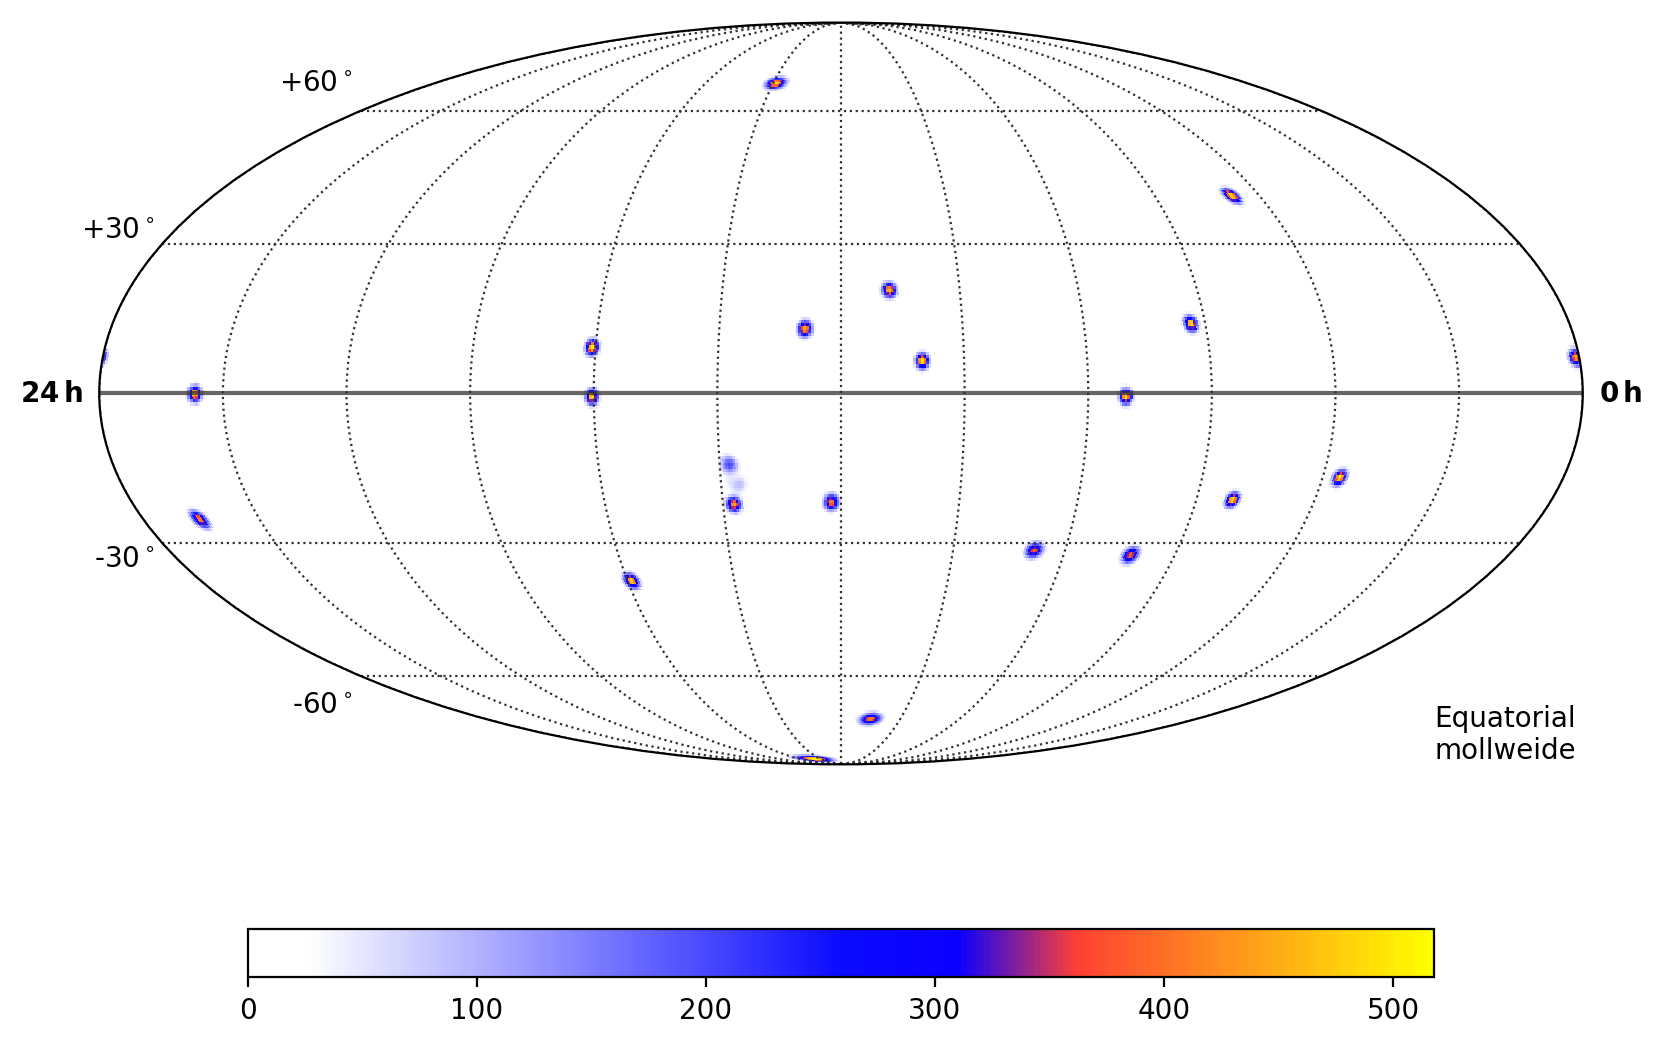
\includegraphics[width=.9\textwidth]{inc/srcs_summed.png}
  \caption{All 22 HESE scan maps in equatorial coordinates. Each map has been converted from log-Likelihood to normal space and smoothed with a 1 degree Gaussian kernel.}
  \label{fig:hese_maps_all}
\end{figure}


\subsection{Test Data}
To test for a neutrino clustering 6 years of point source track data is used.
For this the standardized datasets from skylab are taken from revision 162239.
Matching to the selection of the HESE sources these include
\begin{itemize}
  \item Point Source Tracks \code{'IC79'}
  \item Point Source Tracks \code{'IC86, 2011'}
  \item Point Source Tracks \code{'IC86, 2012-2014'}
  \item GFU \code{"IC86, 2015"}
\end{itemize}
More information on the PS and GFU datasets can be found at the respective analysis wikis: \href{https://icecube.wisc.edu/~coenders/html/build/html/ic86-bdt/muonL3.html}{PS} and \href{https://icecube.wisc.edu/~tkintscher/internal/gfu_doc/eventselection.html}{GFU}.
The data is split in on- and off-time data for blindness reasons, by cutting out the largest time window around all sources.
Usually for time independent analyses the assumption is, that there is far less signal then data in the sample and scrambled data is used to build PDFs for the LLH.
For the tested, small time windows here, we can go a step further and cut out a little bit of data, not biasing the PDF building process, but making sure no sought after signal is incorporated into it.

The HESE events are removed from the on-data, because they αre the reason to test at these positions.

Monte Carlo simulation files are used corresponding to their data counterparts, also taken from skylab's dataset module.
To avoid biased performance and limit estimation, all HESE-like MC events are removed from the used MC sets.
This is done by running the \href{http://software.icecube.wisc.edu/documentation/projects/VHESelfVeto/index.html}{HESE Veto module} on the original MC \code{i3} files.
The actual paths to the files can be found in the script \path{04-check_hese_mc_ids_jobs.py} in the analysis repository.
Surviving run and event IDs are collected and then matched and removed from the used final level files.

Prepared on-, off- and MC-data are stored under \path{/data/user/tmenne/hese_transient_stacking_analysis/rawout_original_hese}.

To built time dependent Likelihood PDfs, run information is needed.
Because no official runlists that match the event selections could be found, run information is reconstructed from data by using the first and last event per run to estimate the runs livetime.
This underestimates the livetime the more the fewer events are in a run.
If a run only had a single event it was dropped.
This doesn't affect on-time data, only the off-data used to build the model PDFs, so a possible single signal event is not cut away in the on-time data.



\section{Analysis Method – Theory}
The analysis is done using an unbinned extended Likelihood method.
THe general idea in the IceCube context is well described in these two overview papers: \href{https://arxiv.org/abs/0801.1604}{Methods for point source analysis in high energy neutrino telescopes} and \href{https://arxiv.org/abs/0912.1572v1}{Time-Dependent Point Source Search Methods in High Energy Neutrino Astronomy}.

\subsection{Extended Unbinned Likelihood}
The extended Likelihood and the corresponding logarithmic extended Likelihood function is defined as
\begin{equation}
  \mathcal{L}(\lambda) = \frac{\lambda^N e^{-\lambda}}{N!}\prod_{i=1}^N P_i
  \quad\Rightarrow\quad
    \ln\mathcal{L}(\lambda) = -\lambda+\sum_{i=1}^N \ln(\lambda P_i)
  \mcomma
\end{equation}
where the constant term $\ln(N!)$ is dropped in the logarithmic version.
Here $\lambda$ is the expected number of events and $N$ the number of measured events following a Poisson counting distribution.
The per event model distribution $P_i$, normalized to integral 1, describes the Likelihood of each event under the assumed model and how likely it contributes to the expectation.
The use of the Poisson term is justified by a renormalization of the per event distributions to include the total number of measured events which is not fixed for multiple experiments of the same kind but may fluctuate around an expectation value.

The tested hypotheses are encoded in the description of the models $P$.
To obtain a fairly general expression we can derive the point source special cases from, we can split the expectation model in multiple classes by splitting the expectation and the models accordingly:
\begin{equation}
  \lambda = \sum_{k=1}^{N_\text{classes}} \lambda_k \geq 0
  \mintertext{and}
  P_i = \frac{1}{\sum_{k=1}^{N_\text{classes}} \lambda_k}\cdot
         \sum_{k=1}^{N_\text{classes}} \lambda_k P_{i,k}
  \mperiod
\end{equation}
The single $\lambda_k$ can be negative but their sum must not because it is still a Poisson expectation parameter.
Additionally we normalized the new split model over all classes and arrive at the form
\begin{equation}
  \ln\mathcal{L}(\{\lambda_k\})
  = -\sum_{k=1}^{N_\text{classes}} \lambda_k +
    \sum_{i=1}^N \ln\left(\sum_{k=1}^{N_\text{classes}}
      \lambda_k P_{i,m} \right)
  \mperiod
\end{equation}

To specialize more, we want to test a signal hypothesis against a background one for $N_\text{srcs}$ sources in general per event $i$.
We thus expand the above expression to include $N_\text{srcs}$ signal and $N_\text{srcs}$ background parameters and the corresponding distributions $S_{i,k}$ and $B_{i,k}$:
\begin{equation}
  \ln\mathcal{L}(\{\lambda_{k,S}\}, \{\lambda_{k,B}\})
  = -\sum_{k=1}^{N_\text{srcs}}\left(\lambda_{k,S}+\lambda_{k,B}\right) +
    \sum_{i=1}^N \ln\left(\sum_{k=1}^{N_\text{srcs}}\left(
      \lambda_{k,S} S_{i,k}+\lambda_{k,B} B_{i,k}\right)\right)
  \mcomma
\end{equation}
and from the Poisson condition we still have the constrain
\begin{equation}
  \sum_{k=1}^{N_\text{srcs}}\left(\lambda_{k,S}+\lambda_{k,B}\right) \geq 0
  \mperiod
\end{equation}

For testing the significance of a potential signal contribution in the measured data, a Likelihood ratio test is used.
The null hypotheses $H_0$, which is that only background is expected to be measured, is constructed by using only a portion $\Theta_0$ of the allowed parameter space, here by setting all signal expectations to zero
\begin{equation}
  \ln\mathcal{L}_0(\{\lambda_{k,S}=0\}, \{\lambda_{k,B}\})
  = -\sum_{k=1}^{N_\text{srcs}}\left(\lambda_{k,B}\right) +
    \sum_{i=1}^N \ln\left(\sum_{k=1}^{N_\text{srcs}}\left(
      \lambda_{k,B} B_{i,k}\right)\right)
  \mperiod
\end{equation}
The alternative hypothesis $H_1$ is constructed using the full Likelihood parameter space $\Theta$:
\begin{equation}
  \ln\mathcal{L}_1(\{\lambda_{k,S}\}, \{\lambda_{k,B}\})
  = -\sum_{k=1}^{N_\text{srcs}}\left(\lambda_{k,S}+
                                     \lambda_{k,B}\right) +
    \sum_{i=1}^N \ln\left(\sum_{k=1}^{N_\text{srcs}}\left(
      \lambda_{k,S} S_{i,k}+\lambda_{k,B} B_{i,k}\right)\right)
  \mperiod
\end{equation}

The Likelihood ratio test statistic $\Lambda$ for testing the null hypothesis $H_0$ against the alternative $H_1$ is defined as
\begin{equation}
  \ln\Lambda = \ln\left(\frac{\sup_{\theta \in \Theta_0} \mathcal{L}(\theta)}
                          {\sup_{\theta \in \Theta} \mathcal{L}(\theta)}\right)
  = \ln\left(\sup_{\theta \in \Theta_0} \mathcal{L}(\theta)\right) -
    \ln\left(\sup_{\theta \in \Theta} \mathcal{L}(\theta)\right)
  \mperiod
\end{equation}

Here we introduce $\hat{\lambda}_{k,S/B}$ which mean the parameters $\lambda_{k,S/B}$ that maximize the Likelihood $\mathcal{L}_1$ under the complete parameter space and $\hat{\lambda}_{k,B}^{(0)}$ maximizing $\mathcal{L}_0$.
This leads to the test statistic
\begin{equation}
  \begin{aligned}
    -2\ln\Lambda
    &= 2\ln(\mathcal{L}_1(\{\hat{\lambda}_{k,S/B}\})) -
       2\ln(\mathcal{L}_0(\{\hat{\lambda}^{(0)}_{k,B}\})) \\
    &= -2\left(\sum_{k=1}^{N_\text{srcs}}\hat{\lambda}_{k,S} +
                                         \hat{\lambda}_{k,B} -
                                         \hat{\lambda}_{k,S}^{(0)}\right) +
      2\sum_{i=1}^N \ln\left(
        \frac{\sum_{k=1}^{N_\text{srcs}}\left(
            \hat{\lambda}_{k,S} S_{i,k}+\hat{\lambda}_{k,B} B_{i,k}\right)}
            {\sum_{k=1}^{N_\text{srcs}}\left(
              \hat{\lambda}_{k,B}^{(0)} B_{i,k}
            \right)}
          \right)
    \mcomma
  \end{aligned}
\end{equation}
which has been decorated by the factor $-2$ to be compatible to Wilks' theorem.
As seen above we have to distinguish all best fit parameters from both hypotheses in general, differentiating $\hat{\lambda}_{k,B}^{(0)}$ from the null hypothesis which are not the same as $\hat{\lambda}_{k,B}$ from the composite hypothesis.

\subsection{Per event distributions}
The introduced per event distributions $S_i, B_i$ are similar for both the time dependent and independent Likelihoods and follow the conventions for most point source searches in IceCube.
These distributions introduce the separation power between signal and background hypotheses in combination with the mixing portions $\lambda_{i,S/B}$ by introducing a-priori knowledge, defining signal- and background-like regions in the parameter space.
The better these distributions are able to separate signal and background regions the more sensitive the analysis becomes.
A common approach with known good separation power is to combine contributions from spatial clustering and energy information, where the first one necessary for the tested hypotheses and the latter providing additional information under certain assumptions of signal flux shapes.
We can then write the signal and background contributions as
\begin{align}
  S_{i,j} &= S(\vec{x}_i, \vec{x}_{\mathrm{src},j}, E_i | \gamma)
    = S^S(\vec{x}_i, \vec{x}_{\mathrm{src},j})\cdot
      S^E(E_i, \delta_i | \gamma) \\
  \intertext{and}
  B_i &= B(\delta_i, E_i | \phi_\mathrm{BG})
    = B^S(\delta_i) \cdot B^E(E_i, \delta_i | \phi_\mathrm{BG})
\end{align}
where $\gamma$ is the shape parameter of an assumed signal flux proportional to a power law $\propto E^{-\gamma}$ and $\phi_\mathrm{BG}$ the usually better known flux model for an atmospheric neutrino flux.

\subsection{Time dependent Likelihood}
To test for time dependent emission we alter our Likelihood similar to what is usually called \enquote{Gamma Ray Burst Likelihood}.
The assumption is, that transient sources have a well defined time window over which neutrino emission might occur.
Here we additionally use non-overlapping time windows so that each source is unique in its own time window.

To account for that, the signal and background PDFs are chosen to include a time part, which is in the most simple case a rectangle function, having only a non-zero contribution at the source's time windows:
\begin{align}
  S_{i,k}^T &= \rect\left(\frac{t_i - \frac{T_k^1-T_k^0}{2}}
                              {T_k^1-T_k^0}\right) \\
  B_{i,k}^T &= \rect\left(\frac{t_i - \frac{T_k^1-T_k^0}{2}}
                              {T_k^1-T_k^0}\right)
  \mcomma
\end{align}
which will be used later.

The other important simplification is that we don't fit the background expectations, but rather fix them from the integrated off-time data rate over the range of the background time PDFs.
This decreases the number of parameters to fit for, unifies the background estimators
\begin{equation}
  \hat{\lambda}_{k,B} = \hat{\lambda}_{k,B}^{(0)} = \Braket{\lambda_{k,B}}
\end{equation}
and the test statistic turns to
\begin{equation}
  \frac{1}{2}\Lambda
  = -\sum_{k=1}^{N_\text{srcs}}\hat{\lambda}_{k,S} +
    \sum_{i=1}^N \ln\left(
      \frac{\sum_{k=1}^{N_\text{srcs}}\hat{\lambda}_{k,S} S_{i,k}}
           {\sum_{k=1}^{N_\text{srcs}}\Braket{\lambda_{k,B}} B_{i,k}}
      + 1 \right)
  \mperiod
\end{equation}

In the following we adapt the notation to the standard and use $n$ instead of $\lambda$.

\subsection{Single sample stacking case}

The stacking test statistic for a single sample now has the form
\begin{align}
  \frac{1}{2}\Lambda
  = -\hat{n}_S + \sum_{i=1}^N \ln\left(\frac{\hat{n}_S\bar{S}_i}{\Braket{n_B} B_i} + 1\right) \mcomma
\label{equ:TS}
\end{align}
where $\hat{n}_S$ is the best fit $n_S$ under the full parameter space and $\bar{S}_i$ the stacked signal PDFs per event at each source $k$
\begin{equation}
  \bar{S}_i = \sum_{k=1}^{N_\text{srcs}} w_k^\text{D} w_k^\text{T} S_{i,k} \mperiod
\end{equation}
The detector weights $w^\text{D}$ and intrinsic source weights $w^\text{T}$ are normalized such that
\begin{equation}
  \sum_{k=1}^{N_\text{srcs}} w^\text{D}_k w^\text{T}_k = 1 \mcomma
\end{equation}
where it doesn't matter if $w^\text{D}$ or $w^\text{T}$ have been normalized on their own or not.

For a single sample and assuming non-overlapping source time windows, we can move the sum over the signal PDFs in eq.~(\ref{equ:TS}) outside the logarithm
\begin{align}
  \frac{1}{2}\Lambda
    &= -\hat{n}_S + \sum_{i=1}^N \ln\left(\frac{\hat{n}_S\bar{S}_i}
                                               {\Braket{n_B} B_i} + 1\right) \\
    &= -\hat{n}_S + \sum_{i=1}^N \ln\left(
          \frac{\hat{n}_S\sum_{k=1}^{N_\text{srcs}}
                w_k^\text{D}w_k^\text{T}S_{i,k}}
               {\Braket{n_B} B_i} + 1\right) \mcomma \\
  \intertext{utilizing that each source has it's unique time window, we see that each event $i$ can only contribute to a single source, so that}
    &= -\hat{n}_S + \sum_{i=1}^N \ln\left(
          \frac{\hat{n}_S\sum_{k=1}^{N_\text{srcs}}
                w_k^\text{D}w_k^\text{T}S_{i,k}\delta_{i\in k}}
               {\Braket{n_B} B_i} + 1\right) \mcomma \\
  \intertext{where $\delta_{i\in k}$ is $1$ only if event $i$ falls into the region of source $k$, otherwise $0$, so we get}
    &= -\hat{n}_S + \sum_{i=1}^N \ln\left(
          \frac{\hat{n}_S
                \left[0 + \dots + 0 +
                      w_k^\text{D}w_k^\text{T}S_{i,k} +
                      0 + \dots + 0\right]}
               {\Braket{n_B} B_i} + 1\right) \mperiod \\
  \intertext{Because $\ln(0+1) = \ln(1) = 0$ we can use this to move the sum outside the logarithm}
    &= -\hat{n}_S + \sum_{k=1}^{N_\text{srcs}}\sum_{i=1}^N \ln\left(
          \frac{\hat{n}_S w_k^\text{D}w_k^\text{T}S_{i,k}}
               {\Braket{n_B} B_i} + 1\right)  \label{equ:single_stack} \\
  \intertext{which, as a crosscheck, expands to the correct expression again:}
    &= -\hat{n}_S + \sum_{i=1}^N \ln\left[
          \ln(1) + \dots + \ln(1) +
          \left( \frac{\hat{n}_S w_k^\text{D}w_k^\text{T}S_{i,k}}
                      {\Braket{n_B} B_i} + 1\right) +
          \ln(1) + \dots + \ln(1) \right] \\
    &= -\hat{n}_S + \sum_{i=1}^N \ln\left[ \left(
          \frac{\hat{n}_S w_k^\text{D}w_k^\text{T}S_{i\in k}}
               {\Braket{n_B} B_i} + 1\right) \right] \mperiod
\end{align}

In the following we'll see, that eq.~(\ref{equ:single_stack}) is already the form we can use to stack over multiple samples.


\subsection{Multiple samples stacking case}

Now if we add another sample, we can just sum up the individual Likelihoods, because they are independent:
\begin{align}
  \frac{1}{2}\Lambda
    &= \frac{1}{2} \sum_{j=1}^{N_\text{sam}} \Lambda_j(\hat{n}_{S,j}) \\
    &= \sum_{j=1}^{N_\text{sam}} \left[
        -\hat{n}_{S,j} + \sum_{k\in j}\sum_{i=1}^{N_j} \ln\left(
          \frac{\hat{n}_{S,j} w_{k,j}^\text{D}w_{k,j}^\text{T}S_{i,k,j}}
               {\Braket{n_B} B_{i,j}} + 1
        \right)
      \right] \\
    &=  -\hat{n}_S + \sum_{j=1}^{N_\text{sam}}
          \sum_{k\in j}\sum_{i=1}^{N_j} \ln\left(
            \frac{\hat{n}_S w_j w_{k,j}^\text{D}w_{k,j}^\text{T}S_{i,k,j}}
                 {\Braket{n_B} B_{i,j}} + 1
        \right) \mperiod
\label{equ:multi_TS}
\end{align}
Here we have individual $n_{S,j}$ signal parameters and sources can exclusively fall in only one of the $N_\text{sam}$ samples.
This is indicated by the sum $\sum_{k\in j}$ over sources now only running over all sources included in sample $j$ and the number of events are now the numbers $N_j$ per sample.
Also the PDFs $S_{i,k,j}$ and $B_{i,j}$ are taken with respect to the sample the source and corresponding events fall into because the PDFs can change depending on the event selection, etc.
Finally, $w_{k,j}^\text{D} w_{k,j}^\text{T}$ are now normalized separately within the sample, so that
\begin{equation}
  \sum_{k\in j} w_{k,j}^\text{D} w_{k,j}^\text{T}
  = \sum_{k\in j} \hat{w}_k^\text{D} \hat{w}_k^\text{T} \cdot
    \frac{1}{\sum_{m\in j} \hat{w}_m^\text{D} \hat{w}_m^\text{T}}
  = 1
  \mperiod
  \label{equ:multi_norm}
\end{equation}

In the last step in eq.~(\ref{equ:multi_TS}) we introduced a weight $w_j$ with
\begin{equation}
  \sum_{j=1}^{N_\text{sam}} w_j = 1 \mcomma
\end{equation}
that scales $\hat{n}_S$ to $\hat{n}_{S,j} = \hat{n}_S w_j$.
We need this to insert the correctly scaled single sample LLH parameters $\hat{n}_{S,j}$ which are in general smaller than the combined $\hat{n}_S$.

To obtain the weights $w_j$ we use the law of total probability
\begin{equation}
  w_j = P(j) = \sum_{k=1}^{N_\text{srcs}} P(j| k)\cdot P(k) \mcomma
\label{equ:tot_prob}
\end{equation}
where $P(j)$ is the probability of getting a signal contribution $\hat{n}_S w_j$ from sample $j$.
$P(j|k)$ is the probability of getting signal from source $k$ from sample $j$, normalized over all samples:
\begin{equation}
  \sum_{j=1}^{N_\text{sam}} P(j|k) = 1 \mperiod
\end{equation}
$P(k)$ is the probability of getting signal from source $k$ at all, normalized over all sources separately:
\begin{equation}
  \sum_{k=1}^{N_\text{srcs}} P(k) = 1 \mperiod
\end{equation}
While eq.~(\ref{equ:tot_prob}) holds in more general cases we can use the assumption about our non-overlapping sources to simplify the expression.
We use matrix notation for eq.~(\ref{equ:tot_prob}) to better illustrate that:
\begin{equation}
  \vec{w} =
    \begin{pmatrix}
      P(j=0|k=0) & \dots & P(j=0|k=N_\text{srcs}) \\
      \vdots & \vdots & \vdots \\
      P(j=N_\text{sam}|k=0) & \dots & P(j=N_\text{sam}|k=N_\text{srcs})
    \end{pmatrix} \cdot
    \begin{pmatrix}
      P(k=0) \\ \vdots \\ P(k=N_\text{srcs})
    \end{pmatrix} \mperiod
\end{equation}

Because each source is assumed to be non-overlapping, each column can only have a single entry which is $1$ after normalization per column.
Each row may contain several entries which in sum are then the number of sources per sample.
The probabilities $P(k)$ can be obtained from the detection efficiency of the detector at the source position in the sample they fall into and are normalized over all sources (see eq.~(\ref{equ:multi_example}) for an example):
\begin{equation}
  \sum_{k=1}^{N_\text{srcs}} P(k)
    = \sum_{k=1}^{N_\text{srcs}} w^\text{D}_k w^\text{T}_k \cdot
      \frac{1}{\sum_{m=1}^{N_\text{srcs}} w^\text{D}_m w^\text{T}_m}
    = 1
  \mperiod
\end{equation}

Because the matrix $P(j|k)$ has only entries with either $1$ or $0$, the weights $w_j$ are effectively the sum over the detection efficiencies of all sources falling in sample $j$
\begin{equation}
  w_j = \sum_{k\in j} w^\text{D}_k w^\text{T}_k
        \frac{1}{\sum_{m=1}^{N_\text{srcs}} w^\text{D}_m w^\text{T}_m}
      \mperiod
\end{equation}
$w^\text{D}_k$ and $w^\text{T}_k$ must not be confused with the weights $w_{k,j}^\text{D}$ and $w_{k,j}^\text{T}$ which are normalized per sample $j$.

But the numerators of the weights $w_j$ are now exactly the normalization of the $w_{k,j}^\text{D}$, $w_{k,j}^\text{T}$ in each sample, as previously seen in eq.~(\ref{equ:multi_norm}):
\begin{equation}
  \text{norm}(\{w_{k,j}^\text{D}w_{k,j}^\text{T}\})
    = \sum_{k\in j} w^\text{D}_k w^\text{T}_k
    = w_j \cdot \sum_{k=1}^{N_\text{srcs}} w^\text{D}_k w^\text{T}_k
  \mperiod
\end{equation}

So if we plug the $w_j$ back in to the test statistic (\ref{equ:multi_TS}) we get
\begin{align}
  \frac{1}{2}\Lambda &=
    -\hat{n}_S + \sum_{j=1}^{N_\text{sam}}
            \sum_{k\in j}\sum_{i=1}^{N_j} \ln\left(
              \frac{\hat{n}_S w_j w_{k,j}^\text{D}w_{k,j}^\text{T}S_{i,k,j}}
                   {\Braket{n_B} B_{i,j}} + 1 \right) \\
    &= -\hat{n}_S + \sum_{j=1}^{N_\text{sam}}
            \sum_{k\in j}\sum_{i=1}^{N_j} \ln\left(
              \frac{\hat{n}_S \left[
                      \frac{\sum_{l\in j} w^\text{D}_l w^\text{T}_l }
                           {\sum_{m=1}^{N_\text{srcs}} w^\text{D}_m w^\text{T}_m}
                      \right] w_{k,j}^\text{D}w_{k,j}^\text{T}S_{i,k,j}}
                   {\Braket{n_B} B_{i,j}} + 1 \right)
       \mperiod \\
  \intertext{The numerator of $w_j$ now cancels the per sample normalization of $w_{k,j}^\text{D}$ and $w_{k,j}^\text{T}$ and we get}
    &= -\hat{n}_S + \sum_{j=1}^{N_\text{sam}}
            \sum_{k\in j}\sum_{i=1}^{N_j} \ln\left(
              \frac{\hat{n}_S \left[
                      \frac{ w_k^\text{D}w_k^\text{T} }
                           {\sum_{m=1}^{N_\text{srcs}} w^\text{D}_m w^\text{T}_m}
                      \right] S_{i,k,j}}
                   {\Braket{n_B} B_{i,j}} + 1 \right)
\end{align}

If we now apply the same arguments about mutually exclusive sources as done in the first part, we can combine the sums over $j$ and $k$ and also just sum over all combined events in all samples $i$.
We then get the test statistic for multiple samples and multiple sources as
\begin{equation}
  \frac{1}{2}\Lambda
  = -\hat{n}_S + \sum_{k=1}^{N_\text{srcs}}\sum_{i=1}^{N} \ln\left(
        \frac{\hat{n}_S \left[
                \frac{ w_k^\text{D}w_k^\text{T} }
                     {\sum_{m=1}^{N_\text{srcs}} w^\text{D}_m w^\text{T}_m}
                \right] S_{i,k}}
             {\Braket{n_B} B_{i, k}} + 1 \right)
   \mcomma
   \label{equ:multi_stack}
\end{equation}
where the index $k$ now means that we have to evaluate the PDFs and the weights with the configuration for the specific sample the source is belonging to.




\section{Analysis Method – Modelling}
Here we want to show the specific choices made to model the per event PDFs for signal and background contribution.
For each we use a combination of independent PDFs for the spatial, energy and time part.

\subsection{Spatial Part}
For the spatial signal PDF a Kent distribution with the per event circular uncertainty $\sigma$ is used.
\begin{equation}
  f(\Psi | \kappa) = \frac{4\pi\sinh\kappa}{\kappa}
    \exp\left(\kappa (\cos\Psi - 1)\right)
\end{equation}
where $\Psi$ is the space angle between the source and event position n equatorial coordinates.
Instead of a $\sigma$ parameter it takes the shape parameter $\kappa$ which can be related by $\kappa \approx 1 / \sigma^2$ for not too large angles $\lesssim 80^\circ$.
A Kent distribution is practically indistinguishable from a 2D Gaussian for small angular uncertainties but is correctly normalized to the unit sphere.

Background PDFs are constructed in equatorial coordinates as well by assuming a flat distribution in azimuth and are estimated under the assumption that the off-time sample contains only background events.
This is only given for larger time windows as the detector location and orientation together with earth's rotation averages out direct detector geometry effects but matters more for small time windows.
Here this is ignored and a flat azimuthal distribution is assumed.

The PDF is thus only declination dependent and can be written as
\begin{equation}
  f_j(\delta) = \frac{1}{2\pi}P(\delta, t_j)
\end{equation}
where $t_j$ is the source time.
A PDF for each source is built considering the sources time and the event distribution at these times to model the different background behaviour due to seasonal variations.
Fig.~(\ref{fig:rate_all_samples}) shows the seasonal variations for the whole sky for all samples.
The steps are:
\begin{enumerate}
  \item For each sample, the events are binned in $\sin\delta$ in 20 bins, with 14 more dense bins around the horizon region, where the event selection usually switches their selection models.
  \item For each bin use the runlists to build $(x|y)$ pairs in time vs. rate information.
  Then rebin that to monthly bins to average out statistical fluctuation for the fit to come.
  \item Fit a sinus function $f(t) = a \sin(b(t-c)) + d$ with free parameters amplitude $a$ and average rate $d$ to the bins to obtain a rate model for each bin.
  The period $2\pi/b$ and the time offset $c$ are fixed to 365 days and to the offset obtained from a full parameter model fit to the whole dataset to fix the beginning of the seasonal variation period
  \item Fit a continuous spline model to these discrete parameter points to obtain a parameter set per source depending on its declination.
  \item To get the background allsky PDF for each sources time window, rate models selected for a fine grid of parameters per declination are selected and integrated over each sources time window.
  The integral points are modelled by an interpolating spline and its integral is renormalized to $\int_{-1}^{1} \mathrm{spl}(\sin\delta) \d{\sin\delta} = 1$.

See fig.~(\ref{fig:dec_bin_rate_models}) for the fitted rate models, fig.~(\ref{fig:param_splines}) for the parameter splines and fig.~(\ref{fig:model_bg_pdfs}) for the resulting background PDFs.

\begin{figure}[h]
  \centering
  \includegraphics[width=.9\textwidth]{inc/rate_models_per_dec_bin/IC86_2012-2014.png}
  \caption{Rate model fits to declination bins for sample IC86, 2012–2014}
  \label{fig:dec_bin_rate_models}
\end{figure}

\begin{figure}[h]
  \centering
  \begin{subfigure}[c]{0.49\textwidth}
    \includegraphics[width=0.9\textwidth]{inc/param_splines/IC86_2012-2014_amp.png}
    \subcaption{Amplitude spline}
  \end{subfigure}
  \hfill
  \begin{subfigure}[c]{0.49\textwidth}
    \includegraphics[width=0.9\textwidth]{inc/param_splines/IC86_2012-2014_base.png}
    \subcaption{Average rate spline}
  \end{subfigure}
  \caption{Rate model parameter splines for amplitude and average rate for sample IC86, 2012–2014. The amplitude spline shows the seasonal variations in the sample.}
  \label{fig:param_splines}
\end{figure}

\begin{figure}[h] % 4 x 3 grid
  \centering
  \begin{subfigure}[c]{0.24\textwidth}
    \includegraphics[width=0.9\textwidth]{inc/sindec_splines/IC86_2012-2014_src_00.png}
  \end{subfigure}
  \hfill
  \begin{subfigure}[c]{0.24\textwidth}
    \includegraphics[width=0.9\textwidth]{inc/sindec_splines/IC86_2012-2014_src_01.png}
  \end{subfigure}
  \hfill
  \begin{subfigure}[c]{0.24\textwidth}
    \includegraphics[width=0.9\textwidth]{inc/sindec_splines/IC86_2012-2014_src_02.png}
  \end{subfigure}
  \hfill
  \begin{subfigure}[c]{0.24\textwidth}
    \includegraphics[width=0.9\textwidth]{inc/sindec_splines/IC86_2012-2014_src_03.png}
  \end{subfigure}

  \begin{subfigure}[c]{0.24\textwidth}
    \includegraphics[width=0.9\textwidth]{inc/sindec_splines/IC86_2012-2014_src_04.png}
  \end{subfigure}
  \hfill
  \begin{subfigure}[c]{0.24\textwidth}
    \includegraphics[width=0.9\textwidth]{inc/sindec_splines/IC86_2012-2014_src_05.png}
  \end{subfigure}
  \hfill
  \begin{subfigure}[c]{0.24\textwidth}
    \includegraphics[width=0.9\textwidth]{inc/sindec_splines/IC86_2012-2014_src_06.png}
  \end{subfigure}
  \hfill
  \begin{subfigure}[c]{0.24\textwidth}
    \includegraphics[width=0.9\textwidth]{inc/sindec_splines/IC86_2012-2014_src_07.png}
  \end{subfigure}

  \begin{subfigure}[c]{0.24\textwidth}
    \includegraphics[width=0.9\textwidth]{inc/sindec_splines/IC86_2012-2014_src_08.png}
  \end{subfigure}
  \hfill
  \begin{subfigure}[c]{0.24\textwidth}
    \includegraphics[width=0.9\textwidth]{inc/sindec_splines/IC86_2012-2014_src_09.png}
  \end{subfigure}
  \hfill
  \begin{subfigure}[c]{0.24\textwidth}
    \includegraphics[width=0.9\textwidth]{inc/sindec_splines/IC86_2012-2014_src_10.png}
  \end{subfigure}
  \hfill
  \begin{subfigure}[c]{0.24\textwidth}
    \includegraphics[width=0.9\textwidth]{inc/sindec_splines/IC86_2012-2014_src_11.png}
  \end{subfigure}

  \caption{Resulting background PDFs for each source in the IC86, 2012--2014 sample. Shown in blue is a spline fit to the grey histogram, which is the averaged PDF over the whole dataset.}
  \label{fig:model_bg_pdfs}
\end{figure}



\end{enumerate}

\subsection{Energy Part}
TODO

\subsection{Time Part}
TODO

\subsection{Fixed Background Estimation and Stacking Weights}
TODO



\section{Analysis Performance}

\subsection{Background Trial Injection}
TODO

\subsection{Signal Trial Injection}
TODO

\subsection{Background Trial Distributions}
TODO

\subsection{Performance}
\subsubsection{Best Case}
TODO
\subsubsection{Realistic Case}
TODO


\section{Analysis Results}



\appendix
\part*{\appendixname}
\section{Presentations}
\begin{description}
  \item[Transients Call] May 22nd, 2017: \href{https://drive.google.com/file/d/0B_Gkg-MCR-1za1RMbjlzTFE0YVU/view}{First Presentation in Transients group}
  \item[Transients Call] June 12th, 2017: \href{https://drive.google.com/file/d/0B_Gkg-MCR-1zTFI3Umg3XzZrSE0/view}{Progress on Software}
  \item[Transients Call] September 18th: \href{https://drive.google.com/file/d/0B_Gkg-MCR-1zR28tTmhBT3VYTGs/view}{Updates on tests on John Felde's NRT analysis}
  \item[Fall Meeting Berlin] October 10th, 2017: \href{https://events.icecube.wisc.edu/getFile.py/access?contribId=37&sessionId=32&resId=0&materialId=slides&confId=90}{First studies on HESE events with PS sample}
  \item[Transients Call] October 30th, 2017: \href{https://drive.google.com/file/d/0B_Gkg-MCR-1zOFdkajczT3JWNUU/view}{Performance and BG trials for all time windows}
  \item[Transients Call] April 30th, 2018: \href{https://drive.google.com/file/d/12vOMOpt1nMrmnBdM_4wV5sMdg0FUJLqF/view}{Update to 6 years of HESE sources}
\end{description}

\section*{Reviewer Q\&A}
\subsection*{Questions from Sandro Kopper -- Collaboration Reviewer}
  \begin{itemize}
      \item Q:
        Concerning the wiki: Better describe spatial PDF, time windows, background injection, rate model fit, used data sets.
      \item A:
        These are addressed with this new version of the analysis documentation.

      \item Q:
        Remove HESE like events from MC data used for performance estimation, because these events would be source positions and not events that are tested for.
      \item A:
        Done.
        I used the \code{VHESelfVeto} module to store all run, event ID combinations of MC events in the \code{i3} files used for the test data sets.
        Then these are removed from the final level MC files used for sensitivity estimation.

      \item Q:
        What happens with the performance if signal is not injected at the best fit HESE positions which are tested?
        The performance should worsen if the sources are not really at the best fit positions.
      \item A:
        Done.
        This is addressed using the healpy injection mode.
        Each trial a new source position is drawn from each prepared millipede scan PDF map and events are injected from these new positions.
        This worsens the sensitivity as expected, the plots and more explanation can be found in the performance section.

      \item Q:
        Make the rate model declination dependent to cover norther, souther sky differences at least.
      \item A:
        Done.
        This was addressed by the method described in the PDF model building section.
        Rate models are fitted to rates in various declination bins and a spline model is used to get a continuous description of the amplitude and average rate per bins.
        These are used to build a background sinus declination PDF for each source separately considering the actual event distribution in the detector at the source's time.

      \item Q:
        Performance for systematics data sets.
      \item A:
        \textcolor{nordorange}{Not done yet}.
        I'm not sure how to do this for the complete analysis.
        For the 7 year PS analysis, the systematics sets were processed for the new selection after IC86 2011 only and also only tested on that subset.
        I could do the same, but that would mean I had to drop all the sources in the IC79 and IC86 sample.
        This is postponed for now, but if someone has some ideas or maybe systematics sets for the missing years, that'd be great.

      \item Q:
        Test time window between the ones actually tested as a cross check.
      \item A:
        \textcolor{nordorange}{Not done yet}, but I think there's not much to see there.
        If required, I can run some BG trials for time windows in between.
  \end{itemize}

\subsection*{Other Questions}
\subsubsection*{Christoph Raab}
  \begin{itemize}
      \item Q (Transients Call, April 30th, 2018):
        What is done with sources that overlap in a different sample?
      \item A:
        There aren't any to consider here, no source is overlapping into another sample even with the largest time window.
        If there would be one, these sources had to be split up to both samples and an additional split weight had to be introduced for injection.
  \end{itemize}

\subsubsection*{Anna Franckowiak}
  \begin{itemize}
      \item Q (Transients Call, April 30th, 2018):
        What motivates the choice for the time windows, why only 5 days, when TXS has shown some 5 months best fit window?
      \item A:
        The windows are chosen somewhat arbitrary.
        The initial decisions to use time windows up to 5 days are that when the analysis started (before TXS), it was not clear how to handle overlapping time windows, so the 5 days provided some buffer to have each source in its unique time window.
        Also, the longer the time window the longer the trial computation takes so this was also a slight factor of not having too large time windows.
  \end{itemize}



\section{Additional Plots}

\begin{figure}[h]
  \centering
  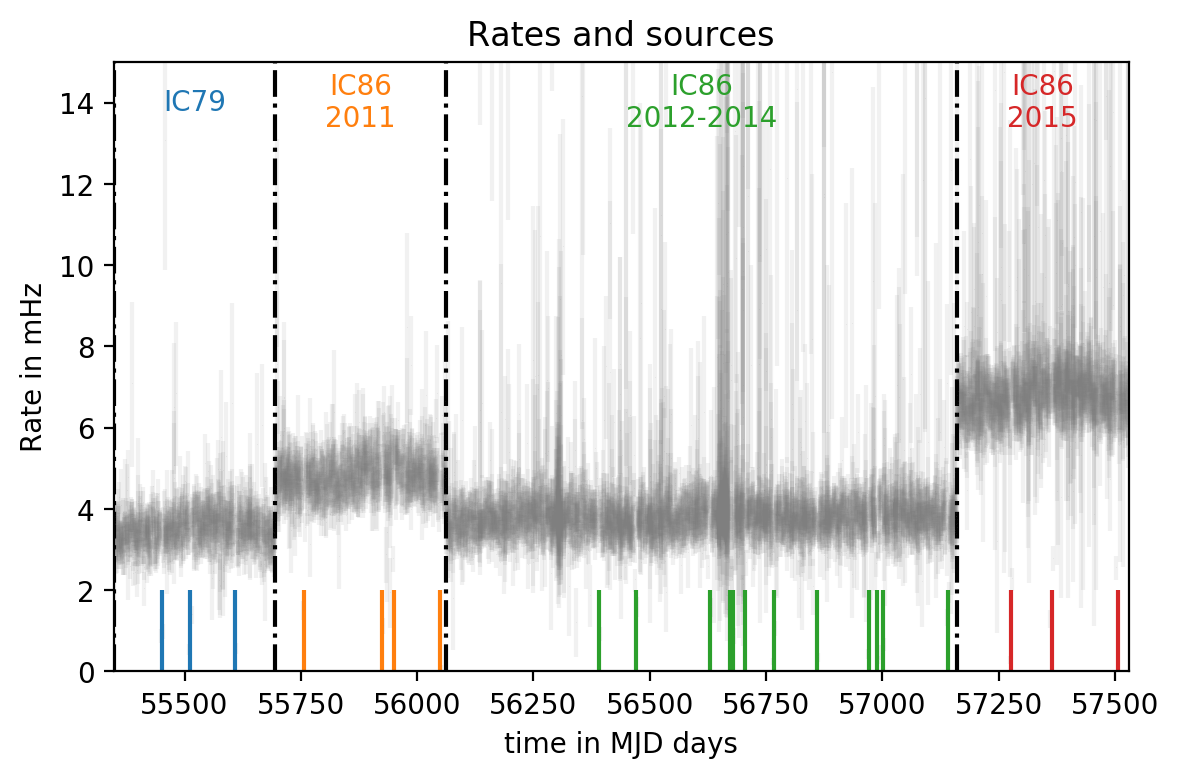
\includegraphics[width=.9\textwidth]{inc/rate_all_samples.png}
  \caption{All runs in the off data samples together with the 22 HESE sources per sample. The rates differ per sample due to different event selections. Seasonal variations cause the sinus like variations per year.}
  \label{fig:rate_all_samples}
\end{figure}


\end{document}